\documentclass{jlreq}

\usepackage{listings}
\usepackage{caption}
\usepackage{fancyhdr}
\usepackage{graphicx}
\pagestyle{fancy}
\fancyhf{} % 既存のヘッダーとフッターをクリア
\fancyhead[R]{\thepage}% 右上にページ番号を配置
\setlength{\headheight}{17.0pt}
\addtolength{\topmargin}{-7.0pt}

\begin{document}
    
\tableofcontents
\clearpage

\section{実験項目}
\subsection{}
オペアンプを用いて電圧フォロワの回路を作成し,電圧フォロワに入力した矩形波および正弦波が
そのまま出力されることをオシロスコープで確認した.

\subsection{}
インダクタ値30mH,抵抗値33\Omega,キャパシタ値2.2{\mu}FのLCRを用いて,LCR回路を作成した.
\begin{figure}
    \centering
    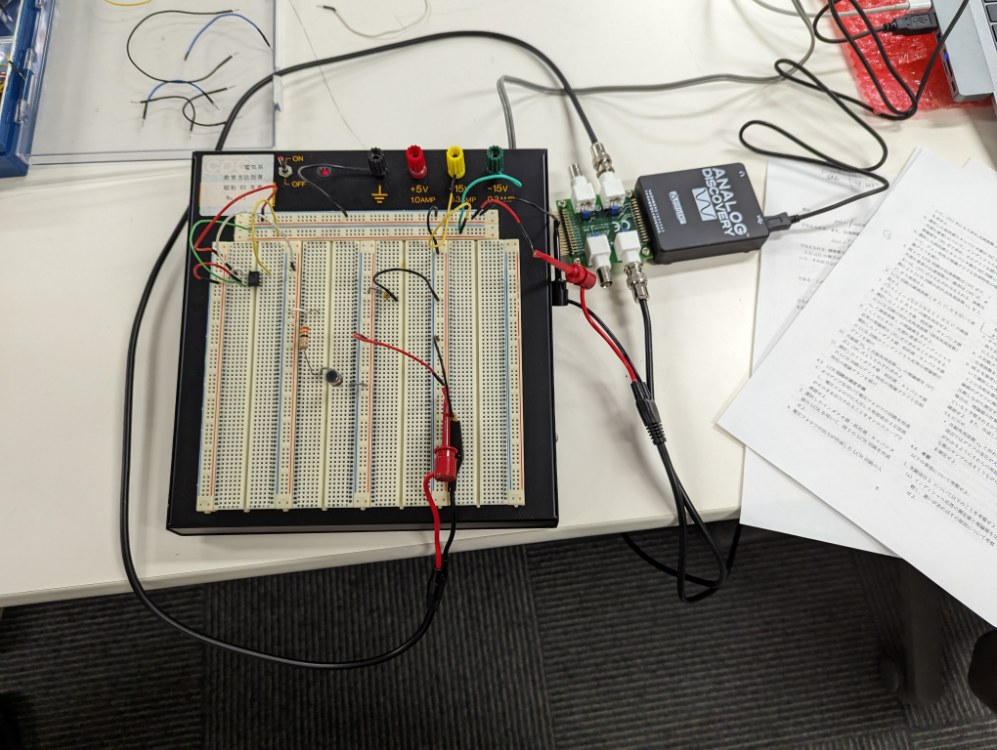
\includegraphics[width=0.5\textwidth]{lcr_circuit.jpg}
    \caption{作成したLCR回路}
    \label{fig:lcr_circuit}
\end{figure}

\subsection{}
電圧フォロワの出力が作成したLCR回路の入力$e_i(t)$となるように接続した.

\subsection{}
信号発生器の出力を矩形波に設定し,その高さを0.5V,オフセットを0.5Vに設定し,0Vから1.0Vで振動する
矩形波が出力されるようにし,その波形をオシロスコープで確認した.

\subsection{}
LCR回路の出力$e_o(t)$が一定値に落ち着くまで表示されるように信号発生器の矩形波の周波数を100Hzに小さくした.

\subsection{}
適当な間隔でLCR回路の出力$e_o(t)$を測定し,理論値のグラフにプロットした.

\section{結果}

\section{考察}
\subsection{実験項目3.について}
\paragraph*{(a)}
\paragraph*{(b)}

\subsection{実験項目4.について}
\paragraph*{(a)}
\paragraph*{(a)}

\section{課題}
\subsection{課題1}

\subsection{課題2}

\subsection{課題3}

\subsection{課題4}

\subsection{課題5}

\end{document}